% Options for packages loaded elsewhere
\PassOptionsToPackage{unicode}{hyperref}
\PassOptionsToPackage{hyphens}{url}
\PassOptionsToPackage{dvipsnames,svgnames,x11names}{xcolor}
\documentclass[
  english,
  12pt,
  a4paper,
]{article}
\usepackage{xcolor}
\usepackage[left=2.5cm,right=2.5cm,top=2.5cm,bottom=2.5cm]{geometry}
\usepackage{amsmath,amssymb}
\setcounter{secnumdepth}{5}
\usepackage{iftex}
\ifPDFTeX
  \usepackage[T1]{fontenc}
  \usepackage[utf8]{inputenc}
  \usepackage{textcomp} % provide euro and other symbols
\else % if luatex or xetex
  \usepackage{unicode-math} % this also loads fontspec
  \defaultfontfeatures{Scale=MatchLowercase}
  \defaultfontfeatures[\rmfamily]{Ligatures=TeX,Scale=1}
\fi
\usepackage{lmodern}
\ifPDFTeX\else
  % xetex/luatex font selection
\fi
% Use upquote if available, for straight quotes in verbatim environments
\IfFileExists{upquote.sty}{\usepackage{upquote}}{}
\IfFileExists{microtype.sty}{% use microtype if available
  \usepackage[]{microtype}
  \UseMicrotypeSet[protrusion]{basicmath} % disable protrusion for tt fonts
}{}
\makeatletter
\@ifundefined{KOMAClassName}{% if non-KOMA class
  \IfFileExists{parskip.sty}{%
    \usepackage{parskip}
  }{% else
    \setlength{\parindent}{0pt}
    \setlength{\parskip}{6pt plus 2pt minus 1pt}}
}{% if KOMA class
  \KOMAoptions{parskip=half}}
\makeatother
% Make \paragraph and \subparagraph free-standing
\makeatletter
\ifx\paragraph\undefined\else
  \let\oldparagraph\paragraph
  \renewcommand{\paragraph}{
    \@ifstar
      \xxxParagraphStar
      \xxxParagraphNoStar
  }
  \newcommand{\xxxParagraphStar}[1]{\oldparagraph*{#1}\mbox{}}
  \newcommand{\xxxParagraphNoStar}[1]{\oldparagraph{#1}\mbox{}}
\fi
\ifx\subparagraph\undefined\else
  \let\oldsubparagraph\subparagraph
  \renewcommand{\subparagraph}{
    \@ifstar
      \xxxSubParagraphStar
      \xxxSubParagraphNoStar
  }
  \newcommand{\xxxSubParagraphStar}[1]{\oldsubparagraph*{#1}\mbox{}}
  \newcommand{\xxxSubParagraphNoStar}[1]{\oldsubparagraph{#1}\mbox{}}
\fi
\makeatother


\usepackage{longtable,booktabs,array}
\usepackage{calc} % for calculating minipage widths
% Correct order of tables after \paragraph or \subparagraph
\usepackage{etoolbox}
\makeatletter
\patchcmd\longtable{\par}{\if@noskipsec\mbox{}\fi\par}{}{}
\makeatother
% Allow footnotes in longtable head/foot
\IfFileExists{footnotehyper.sty}{\usepackage{footnotehyper}}{\usepackage{footnote}}
\makesavenoteenv{longtable}
\usepackage{graphicx}
\makeatletter
\newsavebox\pandoc@box
\newcommand*\pandocbounded[1]{% scales image to fit in text height/width
  \sbox\pandoc@box{#1}%
  \Gscale@div\@tempa{\textheight}{\dimexpr\ht\pandoc@box+\dp\pandoc@box\relax}%
  \Gscale@div\@tempb{\linewidth}{\wd\pandoc@box}%
  \ifdim\@tempb\p@<\@tempa\p@\let\@tempa\@tempb\fi% select the smaller of both
  \ifdim\@tempa\p@<\p@\scalebox{\@tempa}{\usebox\pandoc@box}%
  \else\usebox{\pandoc@box}%
  \fi%
}
% Set default figure placement to htbp
\def\fps@figure{htbp}
\makeatother



\ifLuaTeX
\usepackage[bidi=basic]{babel}
\else
\usepackage[bidi=default]{babel}
\fi
% get rid of language-specific shorthands (see #6817):
\let\LanguageShortHands\languageshorthands
\def\languageshorthands#1{}
\ifLuaTeX
  \usepackage[english]{selnolig} % disable illegal ligatures
\fi


\setlength{\emergencystretch}{3em} % prevent overfull lines

\providecommand{\tightlist}{%
  \setlength{\itemsep}{0pt}\setlength{\parskip}{0pt}}



 
\usepackage[]{natbib}
\bibliographystyle{apalike}


% Text and PDF management
\usepackage{parskip}
\usepackage{setspace}
\usepackage[a-2u]{pdfx}
\hypersetup{hidelinks}
\emergencystretch=1em

% Tables and figures
\usepackage{graphicx}
\usepackage{caption}
\captionsetup[table]{skip=10pt}
\captionsetup{justification=centering}
\usepackage{multirow}
\usepackage{booktabs}
\usepackage{tablefootnote}

% Chemistry and mathematics
\usepackage[version=4]{mhchem}
\usepackage{amsmath}

% Other utilities kept from the original template
\usepackage{lipsum}
\usepackage{datetime}
\newdateformat{mydate}{\THEDAY. \THEMONTH. \THEYEAR}
\renewcommand{\refname}{Reference}
\let\thesisbibliography\bibliography
\renewcommand{\bibliography}[1]{%
  \setstretch{1}%
  \addcontentsline{toc}{section}{Reference}%
  \thesisbibliography{#1}%
}

% Original document spacing
\setlength{\parskip}{10pt}
\setlength{\parindent}{0pt}
\makeatletter
\@ifpackageloaded{caption}{}{\usepackage{caption}}
\AtBeginDocument{%
\ifdefined\contentsname
  \renewcommand*\contentsname{Table of contents}
\else
  \newcommand\contentsname{Table of contents}
\fi
\ifdefined\listfigurename
  \renewcommand*\listfigurename{List of Figures}
\else
  \newcommand\listfigurename{List of Figures}
\fi
\ifdefined\listtablename
  \renewcommand*\listtablename{List of Tables}
\else
  \newcommand\listtablename{List of Tables}
\fi
\ifdefined\figurename
  \renewcommand*\figurename{Figure}
\else
  \newcommand\figurename{Figure}
\fi
\ifdefined\tablename
  \renewcommand*\tablename{Table}
\else
  \newcommand\tablename{Table}
\fi
}
\@ifpackageloaded{float}{}{\usepackage{float}}
\floatstyle{ruled}
\@ifundefined{c@chapter}{\newfloat{codelisting}{h}{lop}}{\newfloat{codelisting}{h}{lop}[chapter]}
\floatname{codelisting}{Listing}
\newcommand*\listoflistings{\listof{codelisting}{List of Listings}}
\makeatother
\makeatletter
\makeatother
\makeatletter
\@ifpackageloaded{caption}{}{\usepackage{caption}}
\@ifpackageloaded{subcaption}{}{\usepackage{subcaption}}
\makeatother
\usepackage{bookmark}
\IfFileExists{xurl.sty}{\usepackage{xurl}}{} % add URL line breaks if available
\urlstyle{same}
\hypersetup{
  pdftitle={Název práce (v ČJ)},
  pdfauthor={Titul. Jméno Příjmení},
  pdflang={en},
  colorlinks=true,
  linkcolor={black},
  filecolor={Maroon},
  citecolor={black},
  urlcolor={black},
  pdfcreator={LaTeX via pandoc}}

\author{Titul. Jméno Příjmení}
\date{}

\begin{document}

\setstretch{1.5}

\begin{titlepage}
\centering
\textbf{Univerzita Karlova}\\
\textbf{Přírodovědecká fakulta}\\[10mm]

Studijní program: Studijní program \break

\begin{figure}[h!]
\begin{center}

\includegraphics[height=8cm]{figures/logo.jpg}
\end{center}
\end{figure}

\textbf{Titul. Jméno Příjmení}\\[1cm]

Název práce (v ČJ)\\[5mm]
Název práce (v AJ)\\[1cm]

Bakalářská práce - Diplomová práce - Rigorózní práce - Disertační práce
- Závěrečná práce v programu celoživotního vzdělávání\\[1cm]

Školitel: \textbf{Jméno školitele}\\
\null\vfill

Praha, \the\year
\end{titlepage}

\pagestyle{empty}
\null\vfill
\noindent Prohlášení
\\[2cm]
Praha, \mydate\today \hfill Autor
\newpage

\null\vfill
\noindent Poděkování
\newpage

\section*{Abstrakt}
Abstrakt

\section*{Klíčová slova}
Klíčová slova
\\

\section*{Abstract}
Abstract

\section*{Keywords}
Keywords

\newpage

\section*{Seznam zkratek}
DFT - Density functional theory
\newpage

\tableofcontents
\newpage

\pagestyle{plain}
\setstretch{1.5}

\section{Introduction}\label{introduction}

\section{Background}\label{background}

\subsection{Spatial statistics}\label{spatial-statistics}

Modelling of spatial phenomena has always been central to geoinformatics
and geographical information science, to the extent that spatial
statistics is considered an integral part of the discipline
\citep{goodchild1992}. As a field, spatial statistics concerns itself
with the quantitative analysis and modelling of spatial data
\citep{pilz2025}, drawing its foundations from probability theory,
mathematical statistics, and stochastic modelling. Its methods address
statistical dependencies between observations, spatial heterogeneity,
and uncertainty inherent to geographic data - using techniques such as
spatial autocorrelation analysis, clustering, interpolation or spatial
modelling among others \citep[\citet{handbook2010}]{ripley1981}.

A common prerequisite to these methods is a mathematically formalized
representation of the relationships between spatial observations. Such
relationships are encoded through spatial weights, which define the
neighbourhood structure of the data and govern how influence is
propagated across space.

This subchapter provides an overview of the core spatial statistical
methods employed in the subsequent analysis. It first introduces spatial
weights with a focus on contiguity definitions, then presents the most
established spatial autocorrelation techniques used to detect
homogeneity and heterogeneity in spatial data. Finally, it discusses
widely used regionalization methods, which seek to partition spatial
units into coherent regions according to attribute similarity and
spatial contiguity constraints.

\subsubsection{Spatial weights}\label{spatial-weights}

Spatial weights, formalized by the seminal work by Cliff \& Ord (1973),
connect objects in geographic space using the spatial relationship
between them. They serve for defining spatial neighbourhoods and
geographically relevant sites. These relationships can be distance-based
(k-nearest neigbours, distance bands), based on a membership in a
geographic group (block weights) or adjacency-based (contiguity) among
others. Each pair of observations is assigned a weight, which can either
be boolean (1 for a spatial relationship, 0 otherwise), or specific
numerical value (e. g. inverse distance). We will further focus on
contiguity-based spatial weights, as those can be directly impacted by
violating polygonal coverage.

Spatial weights can be represented as a matrix, denoted as \(W\). \(W\)
is a \(N \times N\) matrix, where \(N\) is the number observations. Each
element \(w_{ij}\) corresponds to the weight between observations \(i\)
and \(j\), that is, how much observation \(j\) influences observation
\(i\). Because geographic datasets are rarely fully interconnected, most
elements in \(W\) are 0. To ensure computational and memory efficiency,
tools like libpysal \citep{rey2022PySAL}, geoda \citep{anselin2006GeoDa}
or spdep \citep{spdep} also implement sparse matrix, which stores only
non-zero elements.

\begin{figure}

\centering{

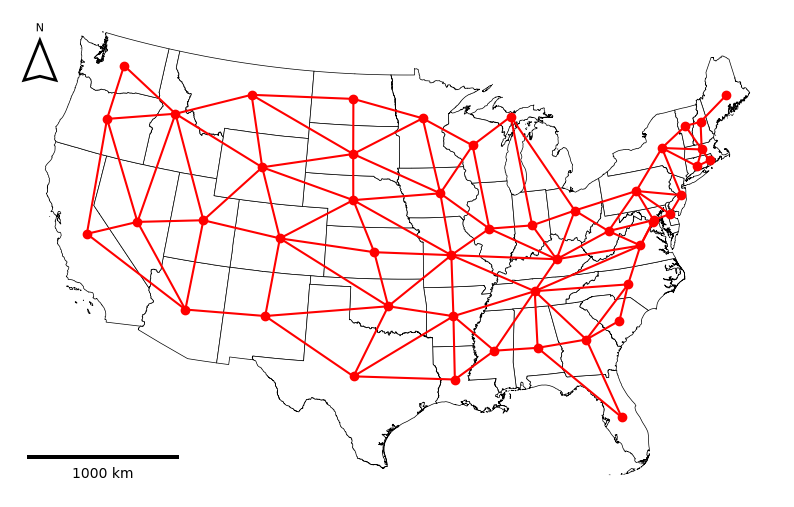
\includegraphics[width=0.8\linewidth,height=\textheight,keepaspectratio]{figures/usa_graph.png}

}

\caption{\label{fig-usa_graph}Rook contiguity graph.}

\end{figure}%

Spatial weight matrix can be understood as a graph adjacency matrix,
therefore spatial graph is another representation of spatial weights. A
weighted graph is defined as an ordered triple \(G = (V,E,\omega)\),
where \(V\) is a set of nodes, \(E\) is a set of edges representing
connectivity between nodes and \(\omega:E \to \mathbb{R}\) is a function
that assigns real numbers (weights) to edges. Two nodes \(i, j \in V\)
are adjacent if there exists an edge \(\{i, j\} \in E\) connecting them.
Each node represents an observation and a weighted edge denotes the
relationship between observations. Fundamentally, spatial weights
matrices and graphs store the exact same topological information; the
matrix is simply the algebraic representation of the spatial graph.

-neco o symetricnosti?

\paragraph{Contiguity}\label{sec-contiguity}

Spatial weight matrices are most commonly defined trough contiguity,
meaning that polygons that share a mutual border are considered to be
spatial neigbours. However, ``sharing a common border'' isn't a rigorous
definition, leading to several formal interpretations of contiguity. The
primary types of contiguity are named analogically to the movements of
chess pieces:

\begin{itemize}
\item
  \emph{Rook}: The polygons are considered neighbours if they share an
  edge (a boundary of non-zero length).
\item
  \emph{Queen}: The polygons are considered neighbours if they share at
  least one point (vertex or a shared edge).
\item
  \emph{Bishop}: The polygons are considered neighbours if they share
  only a point, but no edges. It represents the logical difference
  between \emph{Queen} and \emph{Rook} contiguity (\emph{Queen} -
  \emph{Rook).}
\end{itemize}

Rook and Queen contiguity matrices dominate in spatial statistics. They
are the only valid choice for regionalization methods and are the
default for spatial autocorrelation metrics. Bishop is rarely used on
its own, but sometimes its used for hybrid weights (citace). Beyond
immediate neigbours, contiguty can be expnaded to higer order contiguity
weighs (neigbours of neigbours), often used in spatial data modelling
\citep{floraxImpactsMisspecifiedSpatial1995}.

-nejaky deeper popis contigutiy matrix? symetričnost?

\subsubsection{Spatial autocorrelation}\label{spatial-autocorrelation}

According to Tobler's Firts law of geography ``everything is related to
everything else, but near things are more related than distant things''.
This principle underlies the concept of spatial autocorrelation (SAC) -
the degree to which the value of an observation resembles the values of
its spatial neighbours. Under a positive SAC, observations that are
geographically close have similar values and tend to cluster. Under a
negative SAC, similar values tend to be spatially dispersed rather than
clustered, resembling a checkerboard pattern.

\begin{figure}

\centering{

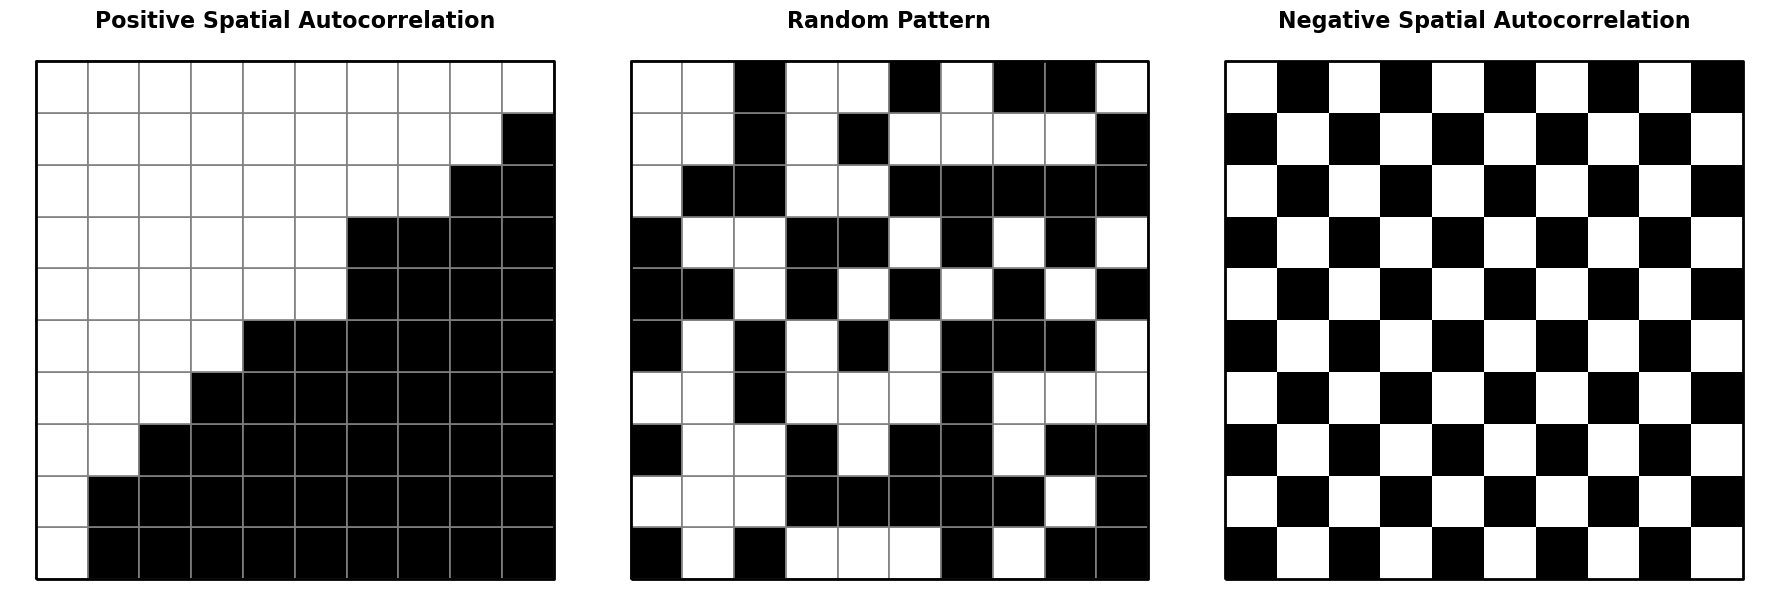
\includegraphics[width=0.8\linewidth,height=\textheight,keepaspectratio]{figures/sac.png}

}

\caption{\label{fig-sac}Spatial autocorrelation.}

\end{figure}%

-spatial autocrrelation pozivame tehdy a tehdy

\paragraph{Moran's I}\label{morans-i}

A useful visualization to built some intuition for SAC is the Moran
scatterplot which visualizes the relationship between the value of each
observation and the values of its neighbour - spatial lag. The spatial
lag of observation \(i\) is the weighted sum of the centered values of
its neighbours, as defined by the spatial weights matrix \(W\):

\begin{equation}\phantomsection\label{eq-lag}{
y_{sl-i} = \sum_{j} w_{ij}y_j
}\end{equation}

where \(w_{ij}\) is an element of \(W\) capturing the spatial
relationship between observations \(i\) and \(j\) and \(y_j\) is the
centered value of observation \(j\). Common pratice is to row
standartize \(W\), so that the weights in each row sum to exactly one.
Neighbours are most commonly defined using either Queen or Rook
contiguity (see Section~\ref{sec-contiguity}).

\begin{figure}

\centering{

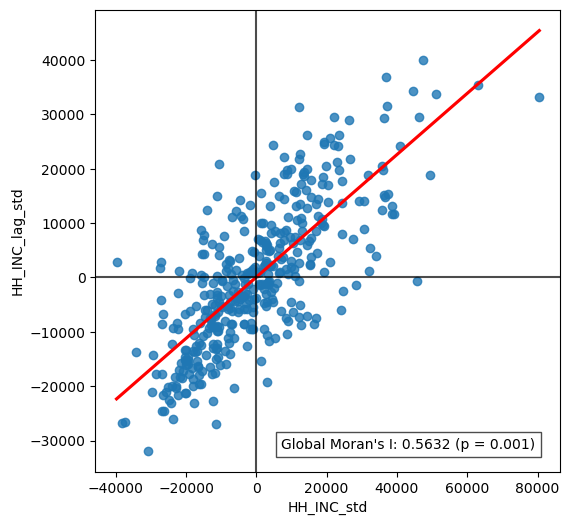
\includegraphics[width=0.6\linewidth,height=\textheight,keepaspectratio]{figures/spatial_lag.png}

}

\caption{\label{fig-moran_scatterplot}Moran's scatterplot.}

\end{figure}%

On the Moran scatterplot, each observation is plotted with its centered
value on the x-axis and its spatial lag on the y-axis. At the global
level, the slope of the best-fit regression line through the scatterplot
corresponds to the value of global Moran's I \citep{moran1950}, the most
widely used SAC statistic. It is defined as

\begin{equation}\phantomsection\label{eq-global_i}{
I = \frac{n}{\sum_i \sum_j w_{ij}} \frac{\sum_i \sum_j w_{ij} z_i z_j}{\sum_i z_i^2}
}\end{equation}

where \(n\) is the number of observations, \(w_{ij}\) is an element of
\(W\) and \(z_i\) and \(z_j\) is the standartized values of observation
\(i\) and \(j\).

The value of \(I\) typically falls within the interval \([-1, 1]\).
Values close to 1 indicate strong positive spatial autocorrelation,
values close to -1 indicate strong negative spatial autocorrelation, and
values close to 0 indicate a spatially random pattern.

At the local level, the four quadrants of the Moran scatterplot
correspond to four characteristic spatial situations, distinguished by
the signs of an observation's value and its spatial lag:

\begin{itemize}
\item
  High-High (HH): an observation with an above-average value surrounded
  by neighbours with above-average values - a cluster of high values.
\item
  Low-Low (LL): an observation with a below-average value surrounded by
  neighbours with below-average values - a cluster of low values.
\item
  Low-High (LH): an observation with an above-average value surrounded
  by neighbours with below-average values - a high-value outlier within
  a low-value neighbourhood.
\item
  High-Low (HL): an observation with a below-average value surrounded by
  neighbours with above-average values - a low-value outlier within a
  high-value neighbourhood.
\end{itemize}

The quadrant to which an observation belongs can be read directly from
the signs of its centered value and its spatial lag. This classification
alone does not indicate whether the observation belongs to that category
because of a genuine spatial pattern or by chance. To make this
distinction, local indicators of spatial association (LISA) are used
together with a test of statistical significance. The most commonly used
local indicator is local Moran's I, defined as

\begin{equation}\phantomsection\label{eq-local_i}{
I_i = \frac{z_i}{m_2} \sum_{j} w_{ij}z_j \; ; \; m_2 = \frac{\sum_i z_i^2}{n}
}\end{equation}

where \(z_i\) and \(z_j\) are centered values on observation \(i\) and
\(j\), \(w_{ij}\) is the spatial weight for a pair of observations \(i\)
and \(j\) and \(m_2\) is the second moment (variance). A positive value
of \(I_i\)\hspace{0pt} indicates that observation \(i\) belongs to an HH
or LL quadrant, whereas a negative value indicates that it belongs to an
HL or LH quadrant.

Because a specific local Moran's I value can be obtained purely by
chance, its statistical significance must be assessed before an
observation is interpreted as belonging to a genuine cluster.
Significance is typically expressed as a p-value under the null
hypothesis that the attribute values are randomly distributed in space
and carry no information about their surroundings. The p-value is
commonly obtained through a permutation procedure, when the observed
values are repeatedly reassigned at random to locations (usually 999
times, esda default), local Moran's I is recalculated for each
permutation, and the p-value is given by the proportion of permutations
producing a value as extreme as, or more extreme than, the observed one.
An observation is conventionally considered a significant part of a
spatial cluster if \(p<0.05\) . In practice, results are often
visualized as LISA cluster maps, in which only statistically significant
HH, LL, HL, and LH clusters are highlighted, while non-significant
observations are shown in grey.

\begin{figure}

\centering{

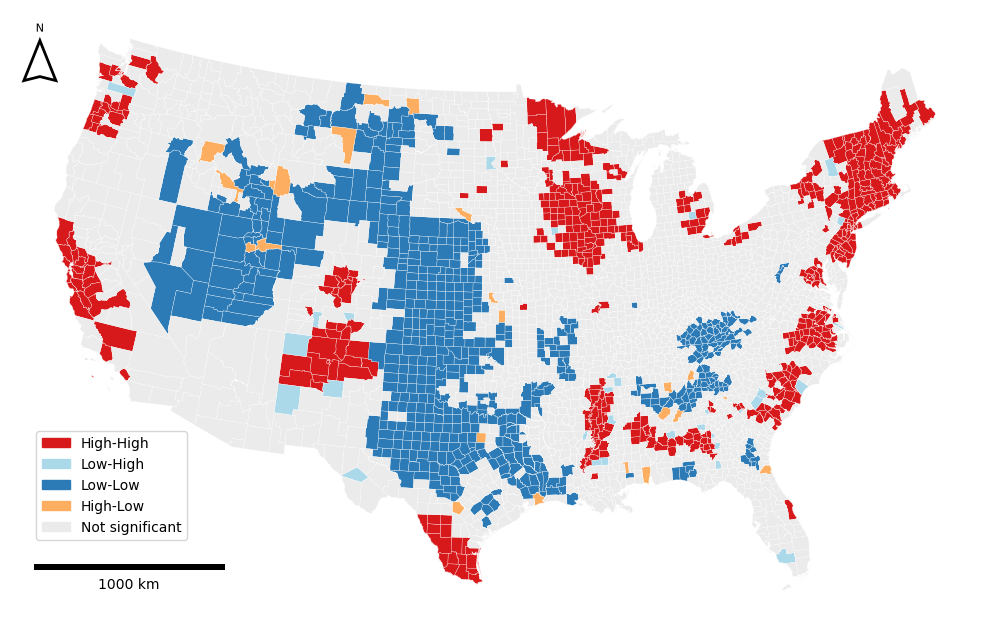
\includegraphics[width=0.8\linewidth,height=\textheight,keepaspectratio]{figures/lisa.png}

}

\caption{\label{fig-lisa_example}LISA cluster map.}

\end{figure}%

On LISA cluster maps of real-world data, the majority of significant
clusters are typically HH or LL, compared to few HL or LH outliers,
which is consistent with Tobler's first law of geography - similar
values tend to occur near one another more often than not.

\paragraph{Geary C}\label{geary-c}

Geary's C is another widely used measure of spatial autocorrelation. Its
global form is given by

\begin{equation}\phantomsection\label{eq-global_c}{
C = \frac{(n - 1)}{2 \sum_i \sum_j w_{ij}} \frac{\sum_i \sum_j w_{ij} (y_i - y_j)^2}{\sum_i (y_i - \bar{y})^2}
}\end{equation}

where \(n\) is the number of observations, \(w_{ij}\) is the spatial
weight for a pair of observation \(i\) and \(j\), \(y_i\) and \(y_j\)
are raw values of observations \(i\) and \(j\), respectively and
\(\bar{y}\) is the mean value of the whole dataset. Unlike Moran's I,
which uses cross-products on the standartized values, Geary's C computes
differences of raw values, which in case of very different neigbouring
values, it inflates the \(C\) value, making it more sensitive to
appearance of local negative SAC. \(C\) is bounded below by zero, which
indicates strong positive SAC, values close to one indicate random
spatial pattern, and any values markably larger than one indicate
negative SAC.

The local version, Local Geary C, proposed by Anselin, is defined for
each observation \(i\) as:

\begin{equation}\phantomsection\label{eq-local_c}{
c_i = \sum_j w_{ij}(y_i - y_j)^2
}\end{equation}

where \(w_{ij}\) is the spatial weight for a pair of observation \(i\)
and \(j\), \(y_i\) and \(y_j\) are raw values of observations \(i\) and
\(j\),. High values of local \(c_i\) highlight areas of abrupt changes
in value. As with any LISA, the magnitude of \(c_i\) is less important
on its own than its statistical significance, which determines whether
the identified local pattern is genuine.

\paragraph{Gettis Ord G}\label{gettis-ord-g}

Proposed by \citet{getis1992}, the local \(G\) is an indicator of
positive spatial autocorrelation. It can be defined in two ways, \(G_i\)
excludes observation's \(i\) own value, wheres \(G_i^*\) includes it:

\begin{equation}\phantomsection\label{eq-local_g}{ G_i = \frac{\sum_{j \neq i} w_{ij} x_j}{\sum_{j \neq i} x_j},G_i^* = \frac{\sum_j w_{ij} x_j}{\sum_j x_j} }\end{equation}

where \(w_{ij}\) is the weight between observation \(i\) and \(j\).
\(G\) captures the overall degree of positive spatial autocorrelation,
where high \(G\) values are associated with hot spots (areas with
homogenously high values) and low values are associated with cold spots
(areas with homogenously low values).

Getis-Ord G is complementary to local Moran's I. Local Moran's I
primarily distinguishes between spatial clusters (HH/LL) and spatial
outliers (HL/LH), but a positive value of local Moran's I does not by
itself reveal whether the underlying cluster consists of high or low
values. \(G\) is specifically designed to make this distinction,
identifying whether a concentration of similar values forms a hot spot
or a cold spot. However, because \(G_i\) and \(G_i^*\)\hspace{0pt} are
computed from sums of raw, non-negative attribute values rather than
centered or standardized ones, they cannot detect negative spatial
autocorrelation.

\subsubsection{Regionalization}\label{regionalization}

Regionalization is the process of creating regions \citep{duque2007}. It
is essentially grouping similar observations together, which we
recognize as clustering, but with a spatial constraint that two
observations (polygons) can be in the same cluster only if they share a
border - contiguity. Regionalization is therefore known as spatially
constrained clustering.

The objective of any clustering method is to minimize the dissimilarity
within each cluster. The overall dissimilarity of a dataset is described
with the sum of all pairwise distances \(T\):

\begin{equation}\phantomsection\label{eq-reg_pairwise_dist}{T = \frac{1}{2} \sum_{i=1}^{n} \sum_{j=1}^{n} d_{ij}}\end{equation}

where \(d_{ij}\) is a measure of dissimilarity. \(T\) consists of two
complementary components: within-cluster dissimilarity \(W\) and
between-cluster dissimilarity \(B\), which can be evaluated during the
clustering (regionalization) process:

\begin{equation}\phantomsection\label{eq-sum_wb}{T=W+B}\end{equation}

where

\begin{equation}\phantomsection\label{eq-wb_explained}{W = \frac{1}{2} \sum_{h=1}^{k} \sum_{i \in h} \sum_{j \in h} d_{ij}, \qquad B = \frac{1}{2} \sum_{h=1}^{k} \sum_{i \in h} \sum_{j \notin h} d_{ij}}\end{equation}

\(W\) acts as a loss function, the goal of clustering is to minimize it.
Some methods explicitly use \(W\) as the clustering criterion (e. g.
SCHC using Ward's linkage) whereas other methods use different metrics
to approximate the goal.

This chapter will serve as an overview of widely used methods discussed
in \citet{anselin2024}. In the experimental part, two of those methods
will be tested for robustness to polygonal coverage violations - SCHC
and SKATER.

\paragraph{SCHC}\label{sec-schc}

Spatially constrained hierarchical clustering (SCHC) is a bottom-up
approach, where each observation starts as its own cluster (\(k=n\)) and
the clusters (or single observations) are being recursively merged based
on their dissimilarity. It is based on agglomerative clustering with a
contiguity constraint. It is a greedy algorithm, therefore once the
observations are merged, they cannot be split in another iteration.

Dissimilarity is computed based on definition of cluster distance in
attribute space, referred to as linkage criterion. The four main types
of linkages are:

\begin{itemize}
\tightlist
\item
  Single linkage: dissimilarity is the minimum distance between any pair
  of observations drawn from the two clusters.
\item
  Complete linkage: dissimilarity is the maximum distance between any
  pair of observations drawn from the two clusters.
\item
  Average linkage: dissimilarity is the average distance over all pairs
  of observations, one drawn from each cluster.
\item
  Ward's linkage: dissimilarity is the increase in total within-cluster
  \(SSD\) (see Equation~\ref{eq-ssd}) that would result from merging the
  two clusters.
\end{itemize}

In vast majority of applications, dissimilarity is measured using
Euclidean distance, which also required for the use of Ward's linkage,
preferred for regionalization and will be further described in this
chapter.

The dissimilarity is denoted in dissimilarity matrix \(D\), which is
initially \(n \times n\) as each observation starts as its own cluster.
Each element \(d_{ij}\) represents the dissimilarity between each pair
of clusters (or single observations). At each step, the algorithm merges
the two clusters/observations, that have the smallest dissimilarity
(smallest value from \(D\)) under the contiguity constraint. After each
merge, \(D\) is updated using an updating formula, that computes the
dissimilarities between the new cluster \(C\) and a cluster \(P\),
reducing both dimensions of \(D\) by one in each iteration.

Ward's method, developed by \citet{ward1963}, explicitly minimizes the
within-cluster dissimilarity (variance) defined trough the sum of
squared errors (\(SSD\)). The input structure to use Ward's method is a
\(n \times p\) matrix \(X\), where \(n\) is the number of observations,
\(p\) is the number of variable and each element represents the
(standartized) value of each variable for each observation. \(SSD\) can
be then formally defined as:

\begin{equation}\phantomsection\label{eq-ssd}{SSD = \sum_{i \in C} (x_i - \bar{x}_C)^2}\end{equation}

where \(x_i\) is a single row of \(X\) (the vector of attributes for
observation \(i\)) and \(\bar{x}_C\) is the centroid of all observations
in cluster \(C\). Intuitively, the overall \(SSD\) increases when we
merge two clusters, so the goal at each step is to choose the merge that
increases \(SSD\) by the smallest possible amount. This turns out to be
equivalent to merging the two clusters whose centroids are closest based
on a dissimilarity matrix \(D\). Ward's method expresses the
dissimilarity trough the square of the Euclidean distance, therefore the
dissimilarity between clusters is defined as

\begin{equation}\phantomsection\label{eq-dissimilarity}{d^2_{AB} = \frac{2n_A n_B}{n_A + n_B} \| \bar{x}_A - \bar{x}_B \|^2}\end{equation}

After two clusters \(A\) and \(B\) are merged into a new cluster \(C\),
the dissimilarities between \(C\) and every other cluster \(P\) can be
computed without recalculating centroids, using the Lance-Williams
updating formula:

\begin{equation}\phantomsection\label{eq-dissimilarity-updating}{d^2_{PC} = \frac{n_A + n_P}{n_C + n_P} d^2_{PA} + \frac{n_B + n_P}{n_C + n_P} d^2_{PB} - \frac{n_P}{n_C + n_P} d^2_{AB}}\end{equation}

As mentioned above, the clusters/observations can be only merged under
the contiguity constraint, which is denoted in spatial weights matrix
\(W\). For this thesis, we will assume a binary \(W\), meaning that
observations \(i\) and \(j\) can be merged only if \(w_{ij}=1\). After
the merge, \(W\) needs to be updated. If \(i\) and \(j\) were merged
into a new cluster \(C\), \(i\)-th and \(j\)-th row and column will be
replaced by \(C\). The relationship between \(C\) and the rest of the
clusters \(P\) will be set to \(w_{PC}= 1\) if
\(w_{iP}=1 \lor w_{jP}=1\), inheriting all the neighbours of both \(i\)
and \(j\).

In practice, the number of clusters (regions) \(k\) is fixed in advance,
and the merging process stops once this number is reached. This
corresponds to ``cutting'' the hierarchical tree refered to as
dendrogram, at the appropriate height.

\begin{figure}

\centering{

\pandocbounded{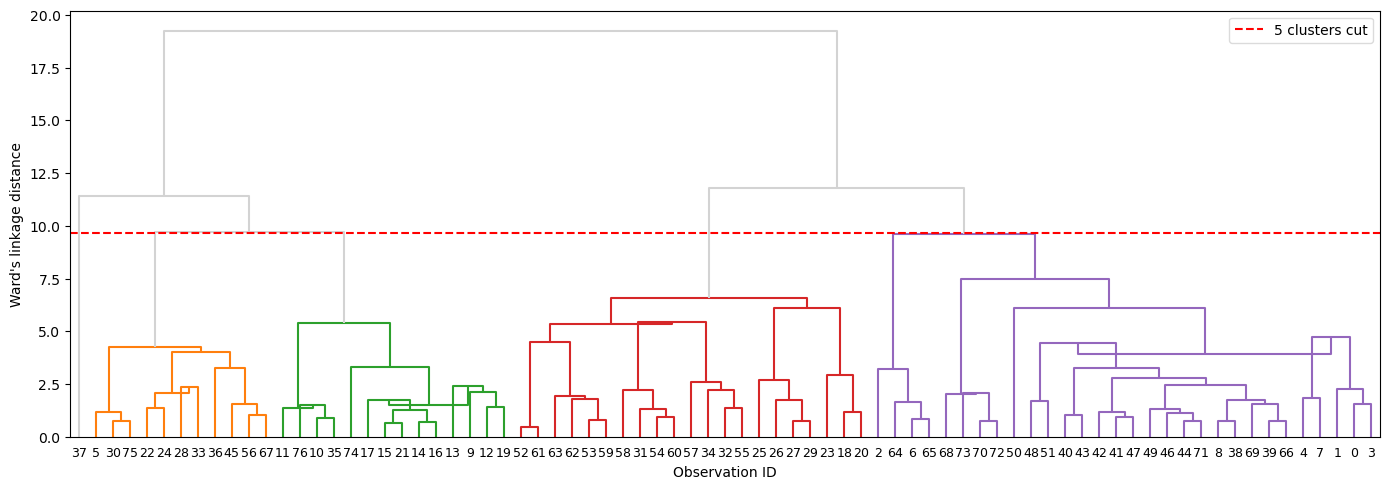
\includegraphics[keepaspectratio]{figures/dendrogram.png}}

}

\caption{\label{fig-dendrgram}Dendrogram.}

\end{figure}%

-definovany jen pro 1 componentu?

\paragraph{SKATER}\label{skater}

Spatial 'K'luster Analysis by Tree Edge Removal (SKATER), developed by
\citet{AssuncaoSkater}, is another hierarchical regionalization method.
Unlike SCHC, it is not agglomerative, but divisive. It is based on
pruning a minimum spanning tree (MST) - a subgraph that connects all
nodes of a graph using the subset of edges with the minimum possible
total edge weight, without forming any cycles. The MST is usually built
using Prim's or Kruskal's algorithm.

\begin{figure}

\centering{

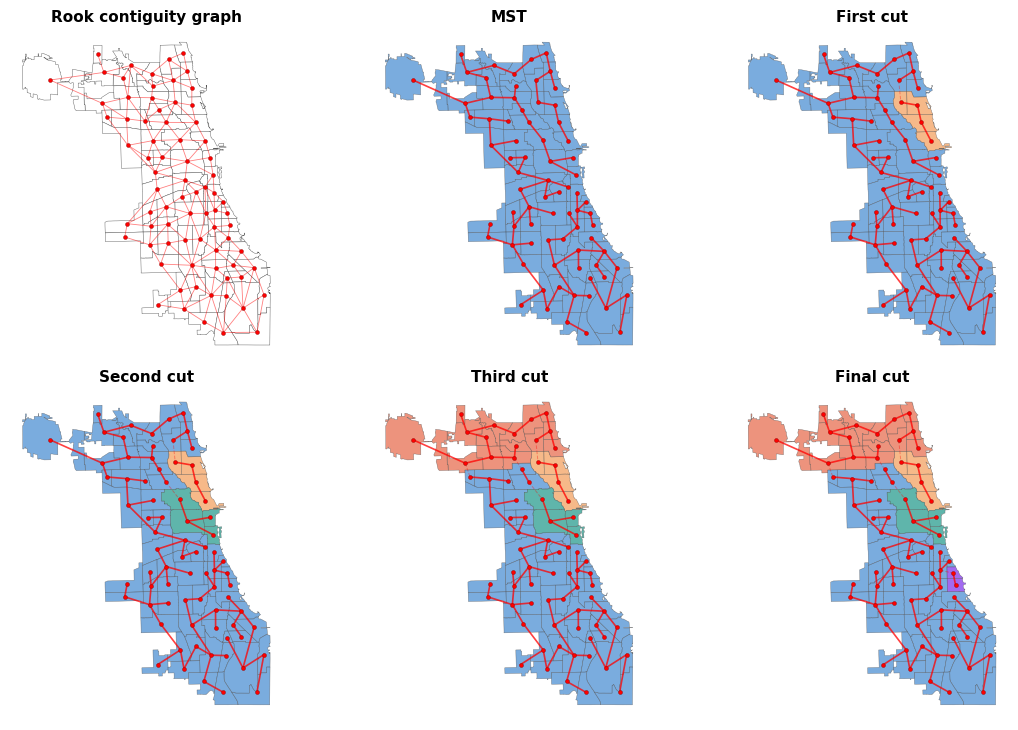
\includegraphics[width=0.8\linewidth,height=\textheight,keepaspectratio]{figures/chicago_skater_steps.png}

}

\caption{\label{fig-skater_partitioning}SKATER partitioning.}

\end{figure}%

For the SKATER algorithm, MST is a subset of edges from contiguity
spatial weights graph (see definiton in Section~\ref{sec-contiguity}).
The weights are assigned to each \((i,j)\) edge based on the
dissimilarity between the attribute vectors of observations \(i\) and
\(j\), typically their squared Euclidean distance in attribute space:

\begin{equation}\phantomsection\label{eq-euclidean_distance_skater}{d(i, j) = d(x_i, x_j) = \sum_{l=1}^{n} (\mathbf{x}_{il} - \mathbf{x}_{jl})^2}\end{equation}

where \(x_i\), \(x_j\) are attribute vectors of observations \(i\) and
\(j\).

All observations are considered to be in one region and they are
connected by the initial MST, which has exactly \(n-1\) edges. The MST
is pruned by removing an edge which increases the between-cluster
dissimilarity the most. This is accessed trough calculating the sum of
squared deviations (see Equation~\ref{eq-ssd}). Removing an edge splits
a tree \(T\) into two subtrees \(A\) and \(B\). The resulting reduction
in within-cluster dissimilarity is given by

\begin{equation}\phantomsection\label{eq-ssd_skater}{\Delta SSD=SSD_T-(SSD_A+SSD_B)}\end{equation}

At each step, SKATER removes the edge that maximizes \(\Delta SSD\),
i.e.~the split that most reduces the combined within-cluster
dissimilarity of the two resulting subtrees. This process is repeated
\(k-1\) times, recursively splitting the resulting subtrees, until the
desired number of regions \(k\) is reached.

\paragraph{REDCAP}\label{redcap}

Developed by \citet{guo2008}, Regionalization with dynamically
constrained agglomerative clustering and partitioning (REDCAP) consists
of both merging and divisive processes, combining SCHC and SKATER.

The first part of the algorithm is structurally identical to SCHC - it
builds an entire dendrogram. It has a dissimilarity matrix, which we can
also think of as a complete graph. That is a graph, that connects all
pairs of possible observations with assigned weight based on their
dissimilarity. The dissmilarity is based on the linkage parameter (see
Section~\ref{sec-schc}). In the original paper, \citet{guo2008} omits
Ward's linkage, though it is implemented in Geoda
\citep{anselin2006GeoDa}.

REDCAP introduces an additional parameter governing which observations
are considered when computing within-cluster dissimilarity. Two
constraining strategies are defined:

\begin{itemize}
\tightlist
\item
  First-order: only edges connecting individual boundary observations
  from different clusters are considered.
\item
  Full-order: All edges connecting observations from different clusters
  are considered. This is equivalent to standard SCHC.
\end{itemize}

During each iteration, the pair of neigbouring clusters that has the
smallest dissimilarity is merged, until all observations belong to one
cluster and a complete dendrogram is built.

More importantly, during this agglomerative process, a MST is
simultaneously constructed. At each iteration, when two clusters are
selected for merging, an edge is added to the MST corresponding to the
minimum-weight edge connecting boundary observations of the two merging
clusters.

After the whole MST is built, the pruning process is the same as in
SKATER, meaning \(k-1\) edges are removed from the MST to reach \(k\)
regions. When REDCAP's First-Order Single-Linkage is used, the MST is
identical the SKATER's one (as well as the resulting regionalization),
as it implicitely uses Kruskal's algorithm.

\paragraph{AZP}\label{azp}

Automatic Zoning Procedure (AZP) was proposed by \citet{openshaw1977}
and extended in \citet{openshaw1995}. Unlike the approaches discussed
above, AZP is not hiearchical. It starts from a complete initial
assignment of all \(n\) observations to \(p\) contiguous regions. For
each region, the within-cluster \(SSD\) is calculated using
Equation~\ref{eq-ssd}. Total within \(SSD\) corresponds to the sum of
all within-cluster \(SSD\)s.

The algorithm randomly picks one of the \(p\) regions (called \(c\)) and
identifies the set \(C\) of all observations that belong to a different
region but are spatially adjacent to at least one observation in \(c\).
From \(C\), an observation \(i\) is randomly selected as a candidate to
leave its current region and join \(c\). For that move to be accepted,
two conditions must be satisfied:

\begin{itemize}
\tightlist
\item
  it must not break the contiguity of \(i\)'s origin region,
\item
  it must decrease the total within-cluster \(SSD\).
\end{itemize}

If both conditions are satisfied, \(i\) is added to region \(c\) and
\(C\) is updated to include any new neighbours introduced by the move.
This process continues until \(C\) is empty. This full cycle over all
regions is repeated from the beginning until a complete pass produces no
accepted swaps, at which point no further improvement in total \(SSD\)
is possible.

AZP does not guarantee a global optimum and can easily become trapped in
a local optimum \citet{anselin2024} . It therefore has several
additional parameters that can improve results. It therefore has several
additional parameters that can improve results. One such parameter is
the \emph{search option}. The default greedy local search only accepts
improving moves. \emph{Tabu search} augments this by maintaining a list
of recently moved observations that are temporarily prohibited from
returning to their origin region, preventing cycling and allowing the
algorithm to escape local optima. \emph{Simulated annealing} uses the
Metropolis algorithm, proposed by \citet{metropolis1953}, to accept
non-improving moves with a probability that decreases over time,
introducing controlled randomness early in the search to escape local
optima while converging towards a stable solution in later iterations.

The other parameter concerns the \emph{initial regionalization}.
\emph{Automatic Regionalization with Initial Seed Location} (ARiSeL)
constructs better initial solutions by selecting seeds based on their
spatial separation and attribute dissimilarity using a K-means++
procedure, rather than relying on random placement. Another option is to
supply the output of a hierarchical method such as SCHC or SKATER as the
starting assignment. Since hierarchical methods cannot rearrange
observations once they are placed in a branch, using their output as an
AZP starting point allows boundary observations to be swapped and the
solution refined \citep{anselin2024}.

\paragraph{Max p-regions problem}\label{max-p-regions-problem}

Proposed by \citet{duque2012}, the max-\(p\) regions problem seeks to
find the maximum number \(p\) of contiguous regions such that each
region meets a minimum size constraint, typically expressed as a lower
bound on a spatially extensive attribute (e.g.~total population).

The heuristic consists of three phases. In the growth phase, an
observation is randomly selected as a seed. Unassigned neighbours are
added one at a time, always choosing the neighbour with the largest
threshold attribute, until the cumulative value of the growing region
meets the threshold. A new seed is then selected and the process
repeats. Any seed whose own attribute value already exceeds the
threshold immediately forms a singleton region. Observations that cannot
be incorporated, because all their neighbours are already assigned or
the minimum bound cannot be reached, are placed in the enclave. The
growth phase is repeated many times from different random starting
points; only the layouts achieving the largest \(p\) are retained.

In the enclave assignment phase, every observation in the enclave is
allocated to a neighbouring existing region so as to minimize the
increase in total within-cluster \(SSD\) (see Equation~\ref{eq-ssd}). If
multiple enclave observations can each join different neighbouring
regions, all combinations are evaluated and the assignment minimizing
total \(SSD\) is chosen.

The outcome of the first two phases is the initial feasible solution,
which is then refined using the same search procedures as AZP - greedy
local search, tabu search, or simulated annealing, to minimize total
\(SSD\) while preserving contiguity and the minimum size constraint. As
with AZP, max-p results are highly sensitive to parameter choices: the
minimum bound value, the number of growth iterations, and the chosen
search strategy, therefore extensive experimentation is recommended
\citep{anselin2024}.

\subsection{Topology in geography}\label{topology-in-geography}

Topology is a mathematical discipline that ``studies properties of
spaces that are invariant to continuous deformation''
\citep{waterloo_topology}. In geographic context, it means focusing
strictly on the spatial relationships between features, such as
connectivity, adjacency, and containment (citace), rather than their
absolute geometric shape, distance, or magnitude.

Topological relationships are essential in numerous geographical
disciplines, such as landscape ecology using overlay analysis, hydrology
and the geography of transport relying on network analysis and line
adjacency, as well as cartography and spatial statistics examining
border topologies \citep{papadimitriou_geo-topology_2023}. Probably one
of the most important connections between topology and geography is the
Four Colour Theorem, proposed by Francis Guthrie in 1852. It states that
any planar map consisting of polygons can be coloured using only four
colours without any pair of neighbouring polygons sharing the same
colour. The theorem was proven more than a hundred years later by
\citet{appel1977fourcolor1}, and it relied entirely on topological
principles, specifically polygonal adjacency.

The formal study topological relationships is rooted in point-set
topology, also known as general topology, as it is the foundation to
many other related disciplines. It relies on the concepts set theory,
introduced by \citet{cantor1874}, like set operations (e. g.
intersection, union, complement), as well as the fundamental notions of
subsets, open sets, and neighborhoods. Furthermore, point-set topology
concepts like interior, boundary and exterior, introduced by
\citet{hausdorff1914grundzuge}, are the foundation for topological
models, used in modern GIS to formalize topological relationships.

This chapter shall explore..

\subsubsection{Topological models}\label{topological-models}

During the 1980s, terms for spatial relations were mentioned in
literature, however, they lacked formal definitions and were mostly
treated as axiomatic \citep{egenhoferPointsetTopologicalSpatial1991}.
The first rigorous framework for topological relationships was the
\emph{4-Intersection Model} (\emph{4-IM}) developed by
\citet{egenhoferPointsetTopologicalSpatial1991}. It applied interior and
boundary definitions from point set topology to a geospatial context.
The \emph{4-IM} served as the predecessor to the \emph{Dimensionally
Extended 9-Intersection Model} (\emph{DE9-IM})
\citep{clementiniSmallSetFormal1993}, which is now the standard adopted
by the \emph{Open Geospatial Consorcium} (\emph{OGC}). Expanding the
\emph{4-IM}, it is based on a 3×3 matrix of all possible intersections
between interior, boundary and exterior of two geometries (point, line
or polygon) and further describes the dimension of those intersections:

\begin{equation}\phantomsection\label{eq-de9im}{\text{DE-9IM}(a,b) = \begin{bmatrix} \dim(a^\circ \cap b^\circ) & \dim(a^\circ \cap \partial b) & \dim(a^\circ \cap b^-) \\ \dim(\partial a \cap b^\circ) & \dim(\partial a \cap \partial b) & \dim(\partial a \cap b^-) \\ \dim(a^- \cap b^\circ) & \dim(a^- \cap \partial b) & \dim(a^- \cap b^-) \end{bmatrix}}\end{equation}

where \(a\) and \(b\) are the input geometries, \(a^\circ\),
\(b^\circ\); \(\partial a\), \(\partial b\); and \(a^-\), \(b^-\) denote
the interior, boundary, and exterior of geometries \(a\) and \(b\),
respectively. The operator \(\cap\) represents the set intersection, and
\(\dim(X)\) returns the maximum topological dimension of the
intersection:

\begin{itemize}
\tightlist
\item
  False (-1) if there is no intersection,
\item
  0 if the intersection is a point,
\item
  1 if the intersection is a line,
\item
  2 if the intersection is a polygon.
\end{itemize}

In most use cases, non-empty intersections (0, 1 or 2) can be
universally treated as \(True\) when the result is invariant to the
intersection dimension. However, for defining contiguities the dimension
of the intersection is required as discussed in
Section~\ref{sec-contiguity}. Specific value combinations in the matrix
have standard names, which are referred to as spatial predicates. The
\emph{C++} library \emph{GEOS} - a core dependency of many libraries (e.
g. \emph{Shapely}, \emph{Geopandas}), databases (e. g. \emph{PostGIS}),
and applications (e. g. \emph{QGIS}) - recognizes 9 spatial predicates
(see tab) \citet{geos}. For computational purposes, the matrix is often
flattened into a 9-character DE-9IM string.

\begin{longtable}[]{@{}
  >{\centering\arraybackslash}p{(\linewidth - 6\tabcolsep) * \real{0.2062}}
  >{\raggedright\arraybackslash}p{(\linewidth - 6\tabcolsep) * \real{0.2062}}
  >{\raggedright\arraybackslash}p{(\linewidth - 6\tabcolsep) * \real{0.1443}}
  >{\raggedright\arraybackslash}p{(\linewidth - 6\tabcolsep) * \real{0.4227}}@{}}
\caption{Spatial predicates. - tohle taky dopnim}\tabularnewline
\toprule\noalign{}
\begin{minipage}[b]{\linewidth}\centering
Spatial predicate
\end{minipage} & \begin{minipage}[b]{\linewidth}\raggedright
DE-9IM string
\end{minipage} & \begin{minipage}[b]{\linewidth}\raggedright
Description
\end{minipage} & \begin{minipage}[b]{\linewidth}\raggedright
Illustration?
\end{minipage} \\
\midrule\noalign{}
\endfirsthead
\toprule\noalign{}
\begin{minipage}[b]{\linewidth}\centering
Spatial predicate
\end{minipage} & \begin{minipage}[b]{\linewidth}\raggedright
DE-9IM string
\end{minipage} & \begin{minipage}[b]{\linewidth}\raggedright
Description
\end{minipage} & \begin{minipage}[b]{\linewidth}\raggedright
Illustration?
\end{minipage} \\
\midrule\noalign{}
\endhead
\bottomrule\noalign{}
\endlastfoot
Intersects & ?? & & \\
Touches & \begin{minipage}[t]{\linewidth}\raggedright
FT*******\\
F**T*****\\
F***T****\strut
\end{minipage} & & \\
Disjoint & FF*FF**** & &
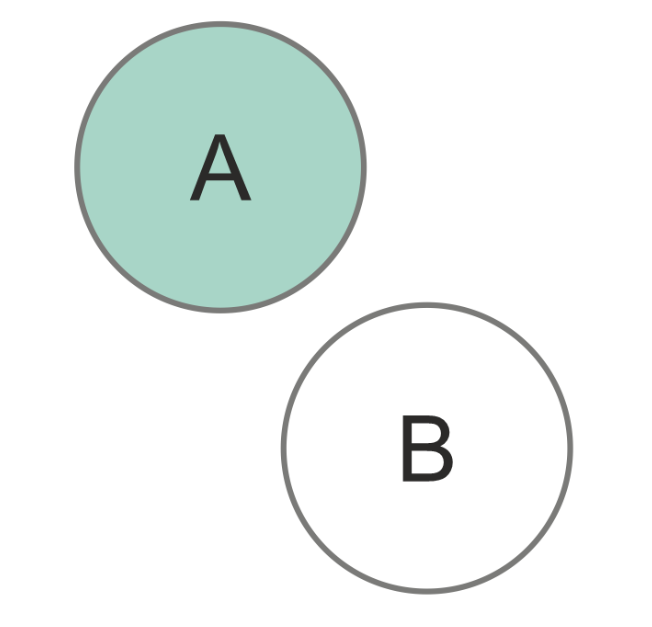
\includegraphics[width=0.3\linewidth,height=\textheight,keepaspectratio]{figures/disjoint.png} \\
Crosses & \begin{minipage}[t]{\linewidth}\raggedright
T*T******\\
0********\strut
\end{minipage} & & \\
Within & T*F**F*** & & \\
Contains & ?? & & \\
Overlaps & T*T***T** & & \\
Equals & TFFFTFFFT & & \\
Covers & ?? & & \\
\end{longtable}

Software libraries implement these predicates alongside additional ones
as boolean functions, such as modified formulations (e. g.
\texttt{contains\_properly()} in \emph{Shapely} library) or inverse
relationships (e. g. \texttt{covered\_by()} in \emph{Shapely}). Custom
spatial queries can be formalized by defining the flattened DE9-IM
string (e. g. \texttt{relate()} in \emph{Shapely}, \texttt{ST\_relate()}
in \emph{PostGIS}). Topological relationships derived from \emph{DE-9IM}
are the underlying framework for many spatial operations including
overlay analysis, contiguity detection, and topology validation.

Because contiguity detection relies directly on the topological
properties of a polygonal dataset, these spatial relationships can be
rigorously defined using the DE-9IM. In libraries such as libpysal,
contiguity is established by evaluating this topological matrix. For
instance, Queen contiguity satisfies the standard \texttt{touches}
spatial predicate. Rook contiguity is defined by the DE-9IM string
\texttt{F***1****}, which mandates that the intersection of the two
polygon boundaries must be exactly 1-dimensional (a shared edge).

\subsubsection{Topological validity and polygonal
coverage}\label{topological-validity-and-polygonal-coverage}

Spatial data often suffers from errors from a variety of sources. These
inaccuracies are typically introduced during manual vectorization or
data entry, data transfer, geometric editing operations (such as
simplification or reprojection), or the integration of heterogeneous
datasets of varying ages \citep[\citet{gisgeography_topology},
\citet{servigne2000}]{spatialeye_topology}.

\citet{servigne2000} categorizes spatial consistency errors into three
primary types:

\begin{itemize}
\tightlist
\item
  \textbf{Structural errors:} Arising when the chosen data structure
  cannot adequately accommodate the data model.
\item
  \textbf{Geometric errors:} Conceptually invalid geometry (e. g.
  self-intersecting polygons).
\item
  \textbf{Topo-semantic errors:} Occurring when the geometric
  representation violates real-world logical constraints (e.g., a single
  building footprint incorrectly intersecting two distinct parcels).
\end{itemize}

Geometric and topo-semantic errors are particularly problematic when
detecting topological relationships, as they are not immediately
noticable. The most commonly used data structures in modern GIS are
``spaghetti'' models (e.g., GeoJSON, Shapefile, Parquet, and
GeoPackage). These models store each geometry as an isolated record with
no information about their mutual relationships, therefore they need to
be derived from the geometry (vertices). In presence of geometrical
inaccuracies, accurate detection of topological relationships is
impossible.

According to \citet{ubedaTopologicalErrorCorrecting1997a}, the topology
error correction process consists of three steps: definition, checking,
and correction. Definitions of the errors is esentially establishing the
spatial constraints input data must satisfy. These user-defined
constraints are derived from formal spatial predicates. Many of these
rules are explicitely implemented as ready-to-use topology checkers in
desktop GIS software like \emph{QGIS} and \emph{ArcGIS Pro} (e. g.
\texttt{must\ not\ have\ dangles} for line features,
\texttt{must\ not\ overlap} for line or polygonal features).

\paragraph{Polygonal coverage}\label{polygonal-coverage}

Polygonal coverage, or also planar enforcement, is a specific selection
of topology rules. It is a strict requirement for contiguity detection
\citep{rey2022PySAL}. Geoplanar \citep{geopanda2026}, a python package
developed for planar enforcement of Geopandas datasets, considers five
planar enforcement violations, see table/fig.

-fig violations and names

\textbf{Overlaps} occur when two polygons share part of their interior.
They are identified using the \texttt{overlaps} spatial predicate, which
returns an array of index pairs corresponding to overlapping geometries.
The violation can be resolved either by trimming one of the polygons to
remove the shared area, or by merging the two polygons into one.

\textbf{Gaps} are detected by converting polygon boundaries to
linestrings and exploiting a key property of planar enforcement: when
two polygons share an edge perfectly, their coincident boundaries merge
into a single linestring after \texttt{union\_all()}. Where a gap
exists, the edges do not coincide and remain as separate LineStrings,
enclosing the void between them. \texttt{polygonize} then reconstructs
every closed face from this line network, producing both the original
polygons and any gap polygons as closed faces. The resulting set is
filtered against the original GeoDataFrame using the \texttt{covers}
predicate --- gap polygons are not covered by any input polygon, since
no input geometry claims that space.

\textbf{Omitted interiors} arise when a polygon lies entirely within
another polygon, meaning the larger polygon should contain a hole, but
none is encoded in its geometry. They are identified using the
\texttt{contains} spatial predicate. The violation is corrected by
subtracting the smaller polygon from the larger one, punching a
correctly encoded hole into the larger geometry.

In presence of \textbf{non-planar edges and touches}, contiguity
detection is compromised. \emph{Rook} contiguity considers two polygons
neighbours if they share at least two consecutive vertices, and those
vertices must be explicitly present and encoded in both polygons,
stricter than a pure spatial predicate testing for overlapping
boundaries. \emph{Queen} contiguity similarly requires a shared vertex
to exist in both geometries. Geoplanar detects violations by subtracting
a \emph{Queen} contiguity graph from a fuzzy contiguity graph, where
fuzzy contiguity captures geometrically adjacent pairs regardless of
shared vertex encoding. Pairs that appear in the fuzzy graph but not in
the \emph{Queen} graph are flagged as non-planar. The violation is
corrected by inserting additional vertices into the relevant geometries,
ensuring that every shared edge is encoded with a consistent set of
vertices on both sides.

-fig non planar touches/edges

-identifying a Fixing errors, trosku detailneji se zamerit na geoplanar
a pak zminit dalsi (qgis/arcgis, mapshaper, jts)

Fuzzy contiguity \citep{rey2022PySAL} doesn't change the geometry of
polygons, but it is a tool to generate \(W\) without requiring strict
topological relationships. By default, it creates a buffer (automatic or
user-specified) around the polygonal geometries. Buffered polygons, that
meet the spatial predicate \texttt{intersects} (by default) are then
considered to be neighbours and this relationship is denoted in \(W\).

-diagram pro premka

-even though such tools exist, topological errors still occur, a presne
proto pisu tuhle praci

\subsubsection{Erroneous datasets??}\label{erroneous-datasets}

\subsection{Related work}\label{related-work}

A critical gap in the current literature is the lack of research
explicitly isolating the direct impact of topological errors on spatial
statistical methods. This literature review chapter is dedicated to
conceptually and methodologically similar studies. First, it introduces
the broader landscape of spatial data uncertainty and errors, and their
impact. Next, it discusses the specification of spatial weights matrices
and its impacts on spatial analysis. Afterwards, it looks at the
behaviour of spatial statistical methods under specific data conditions,
such as .. Lastly, it focuses on graph degradation, which in the context
of spatial weights is omitted in the literature, however, it is used in
simulating road network disruption among others.

\subsubsection{Data uncertainty}\label{data-uncertainty}

\citet{fisher1999models} distinguishes three primary forms of
uncertainty in spatial data: error, vagueness, and ambiguity. Error
occurs when a geographical object is well-defined, but its recorded
measurement or position deviates from the objective truth. Vagueness
arises when the boundaries of an object are not clearly defined or
crisp. Finally, ambiguity happens when there are multiple differing
definitions or classifications for a single object or attribute, an
issue fundamentally tied to subjective human interpretation.

-this thesis focuses on the error part

To address positional uncertainty in spatial optimization,
\citet{wei2012} introduced the multi-objective Error-Anti-Covering
Location Problem (E-ACLP) to evaluate sex offender residency dispersion
laws, which require a mandatory 1,320-foot separation distance
\(\Gamma\) between households. The E-ACLP embeds a \(\pm\) 100-foot
geographic error margin \(\epsilon\) by mathematically partitioning
proximity constraints into a \emph{certain conflict set} (less than
\(\Gamma - \epsilon\)) and an \emph{uncertain conflict set} (between
\(\Gamma - \epsilon\) and \(\Gamma + \epsilon\)). The model then
maximizes total legal residences while minimizing a penalty function
that charges a uniform cost of 1 for every uncertain constraint it is
forced to relax. The results demonstrate that while an error-blind model
identifies an upper bound of 16 residences, the E-ACLP maps a risk
spectrum from an ultra-conservative 15 residences up to an aggressive 19
residences, revealing that maximizing capacity to 19 requires accepting
22 potential proximity violations.

@wei2022, \citet{murray2012}, \citet{heuvelink1998},
\citet{uncertai2015}, \citet{griffith2018}

Several studies adress the impact of positional error on change
detection, generating ``false change''. This false change is attributed
to sliver polygons, caused by boundary misalignments between compared
datasets across two time periods, which fundamentally represent a form
of topological error. \citet{mas2005} employed a probabilistic epsilon
band \citep[\citet{chrisman}]{perkal1956epsilon} around boundaries,
classifying any change polygon falling completely within it as false
change. When applied to a synthetic dataset with zero true change, this
method successfully eliminated 95\% of the artificially generated sliver
polygons, though the author cautions that excessively wide bands risk
erasing narrow, legitimate geographic features. Moving beyond uniform
error assumptions, \citet{declercq2009} utilized Monte Carlo simulations
and piecewise rubber-sheeting to prove that the severity of this
boundary corruption is strictly governed by landscape geometry,
identifying edge density and the number of patches as the primary
drivers of vulnerability.

-mozna nejaky networks

\subsubsection{Specification of weight
matrix}\label{specification-of-weight-matrix}

Weight matrix choice is pretty well researched in literature.
\citet{wei2012}

It has been mostly studied of spatial autocorrelation and spatial
autoregressive models.

\citet{lesage2010} refer to to the fact that misspecification of weight
matrix can severly impact the estimates ans inferences as ``biggest myth
in spatial econometrics''.

\subsubsection{Reliability of spatial analysis in specific
conditions}\label{reliability-of-spatial-analysis-in-specific-conditions}

-testovani na divnejch datech, \citet{westerholt_social_media},
\citet{westerholt_poisson}, \citet{westerholt_interference}

\subsubsection{Graph degradation}\label{graph-degradation}

-graph corruption (mostly silnice)

\section{Methodology}\label{methodology}

\begin{figure}

\centering{

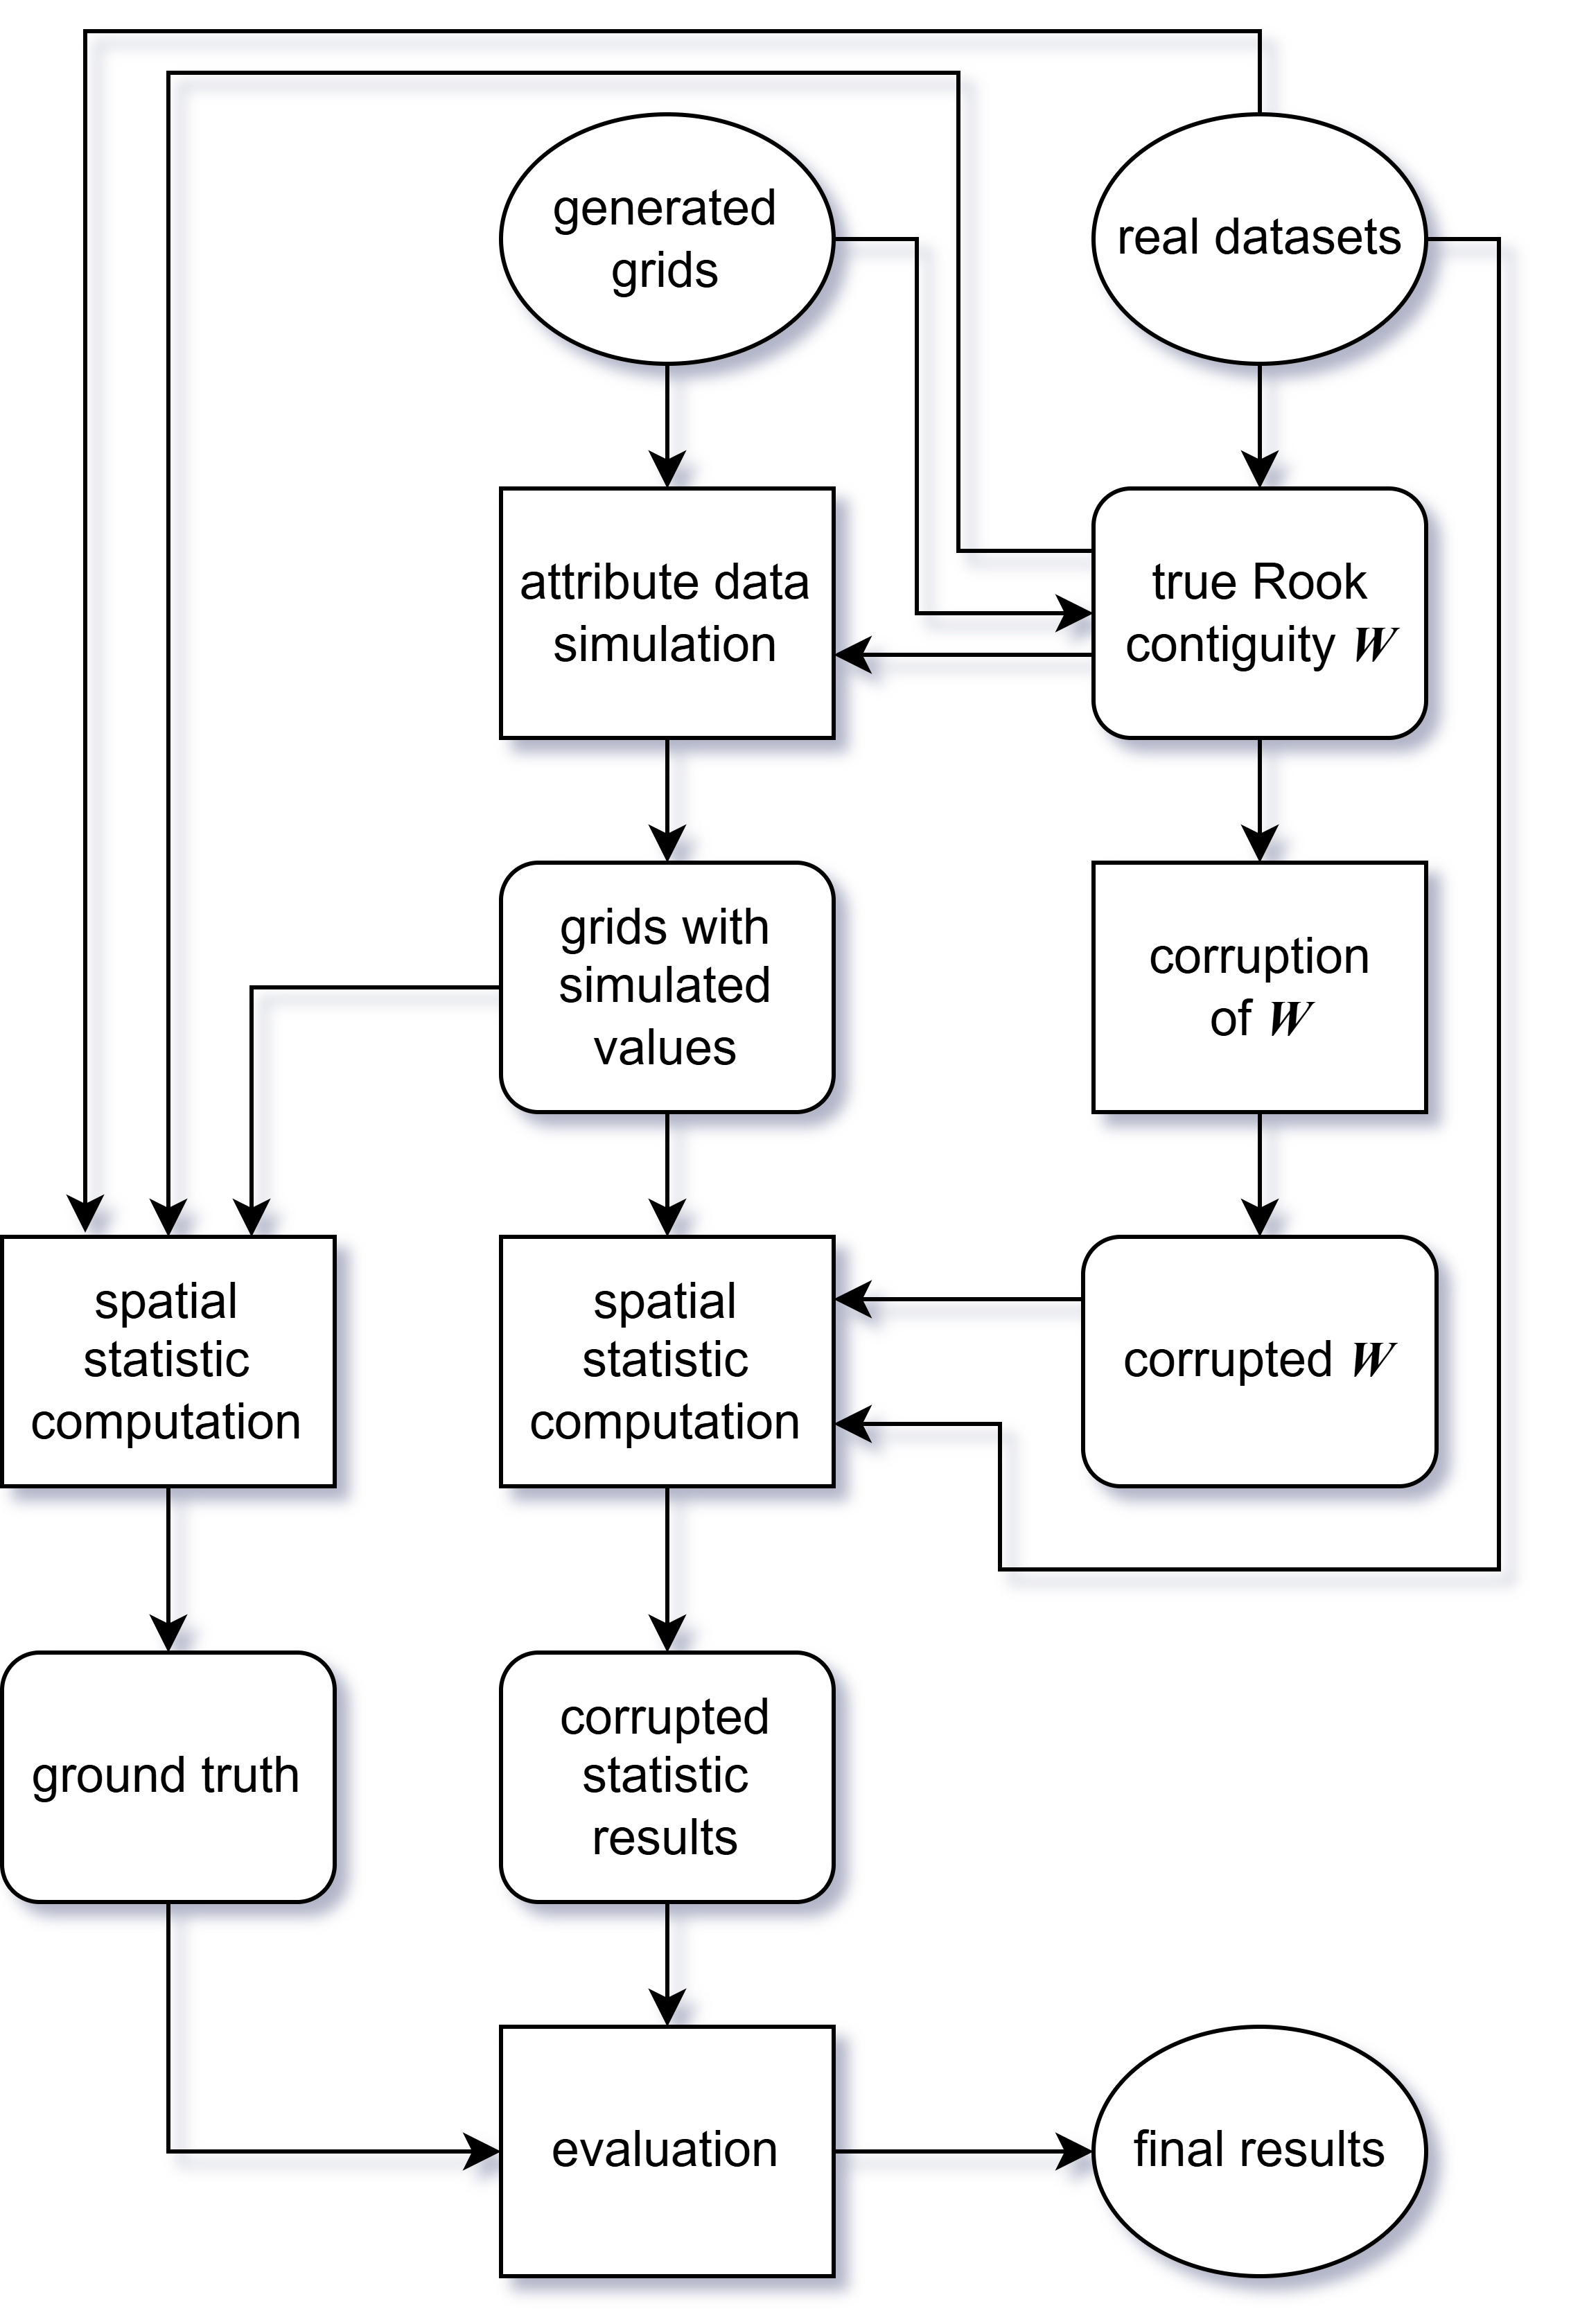
\includegraphics[width=0.5\linewidth,height=\textheight,keepaspectratio]{figures/overall_draw.png}

}

\caption{\label{fig-overall_pipeline}Methology pipeline.}

\end{figure}%

\subsection{Grid generation}\label{grid-generation}

To test robustness of spatial statistics under supervised conditions,
three lattice geometries were considered - square, pentagonal (A5) and
hexagonal (H3). Lattice geometry influences the number of average number
of neigbours per observation. All three geometries were generated in
three different dataset sizes - \(n=25\) (5×5 grid), \(n=100\) (10×10
grid), and \(n=400\) (20×20 grid).

\begin{figure}

\centering{

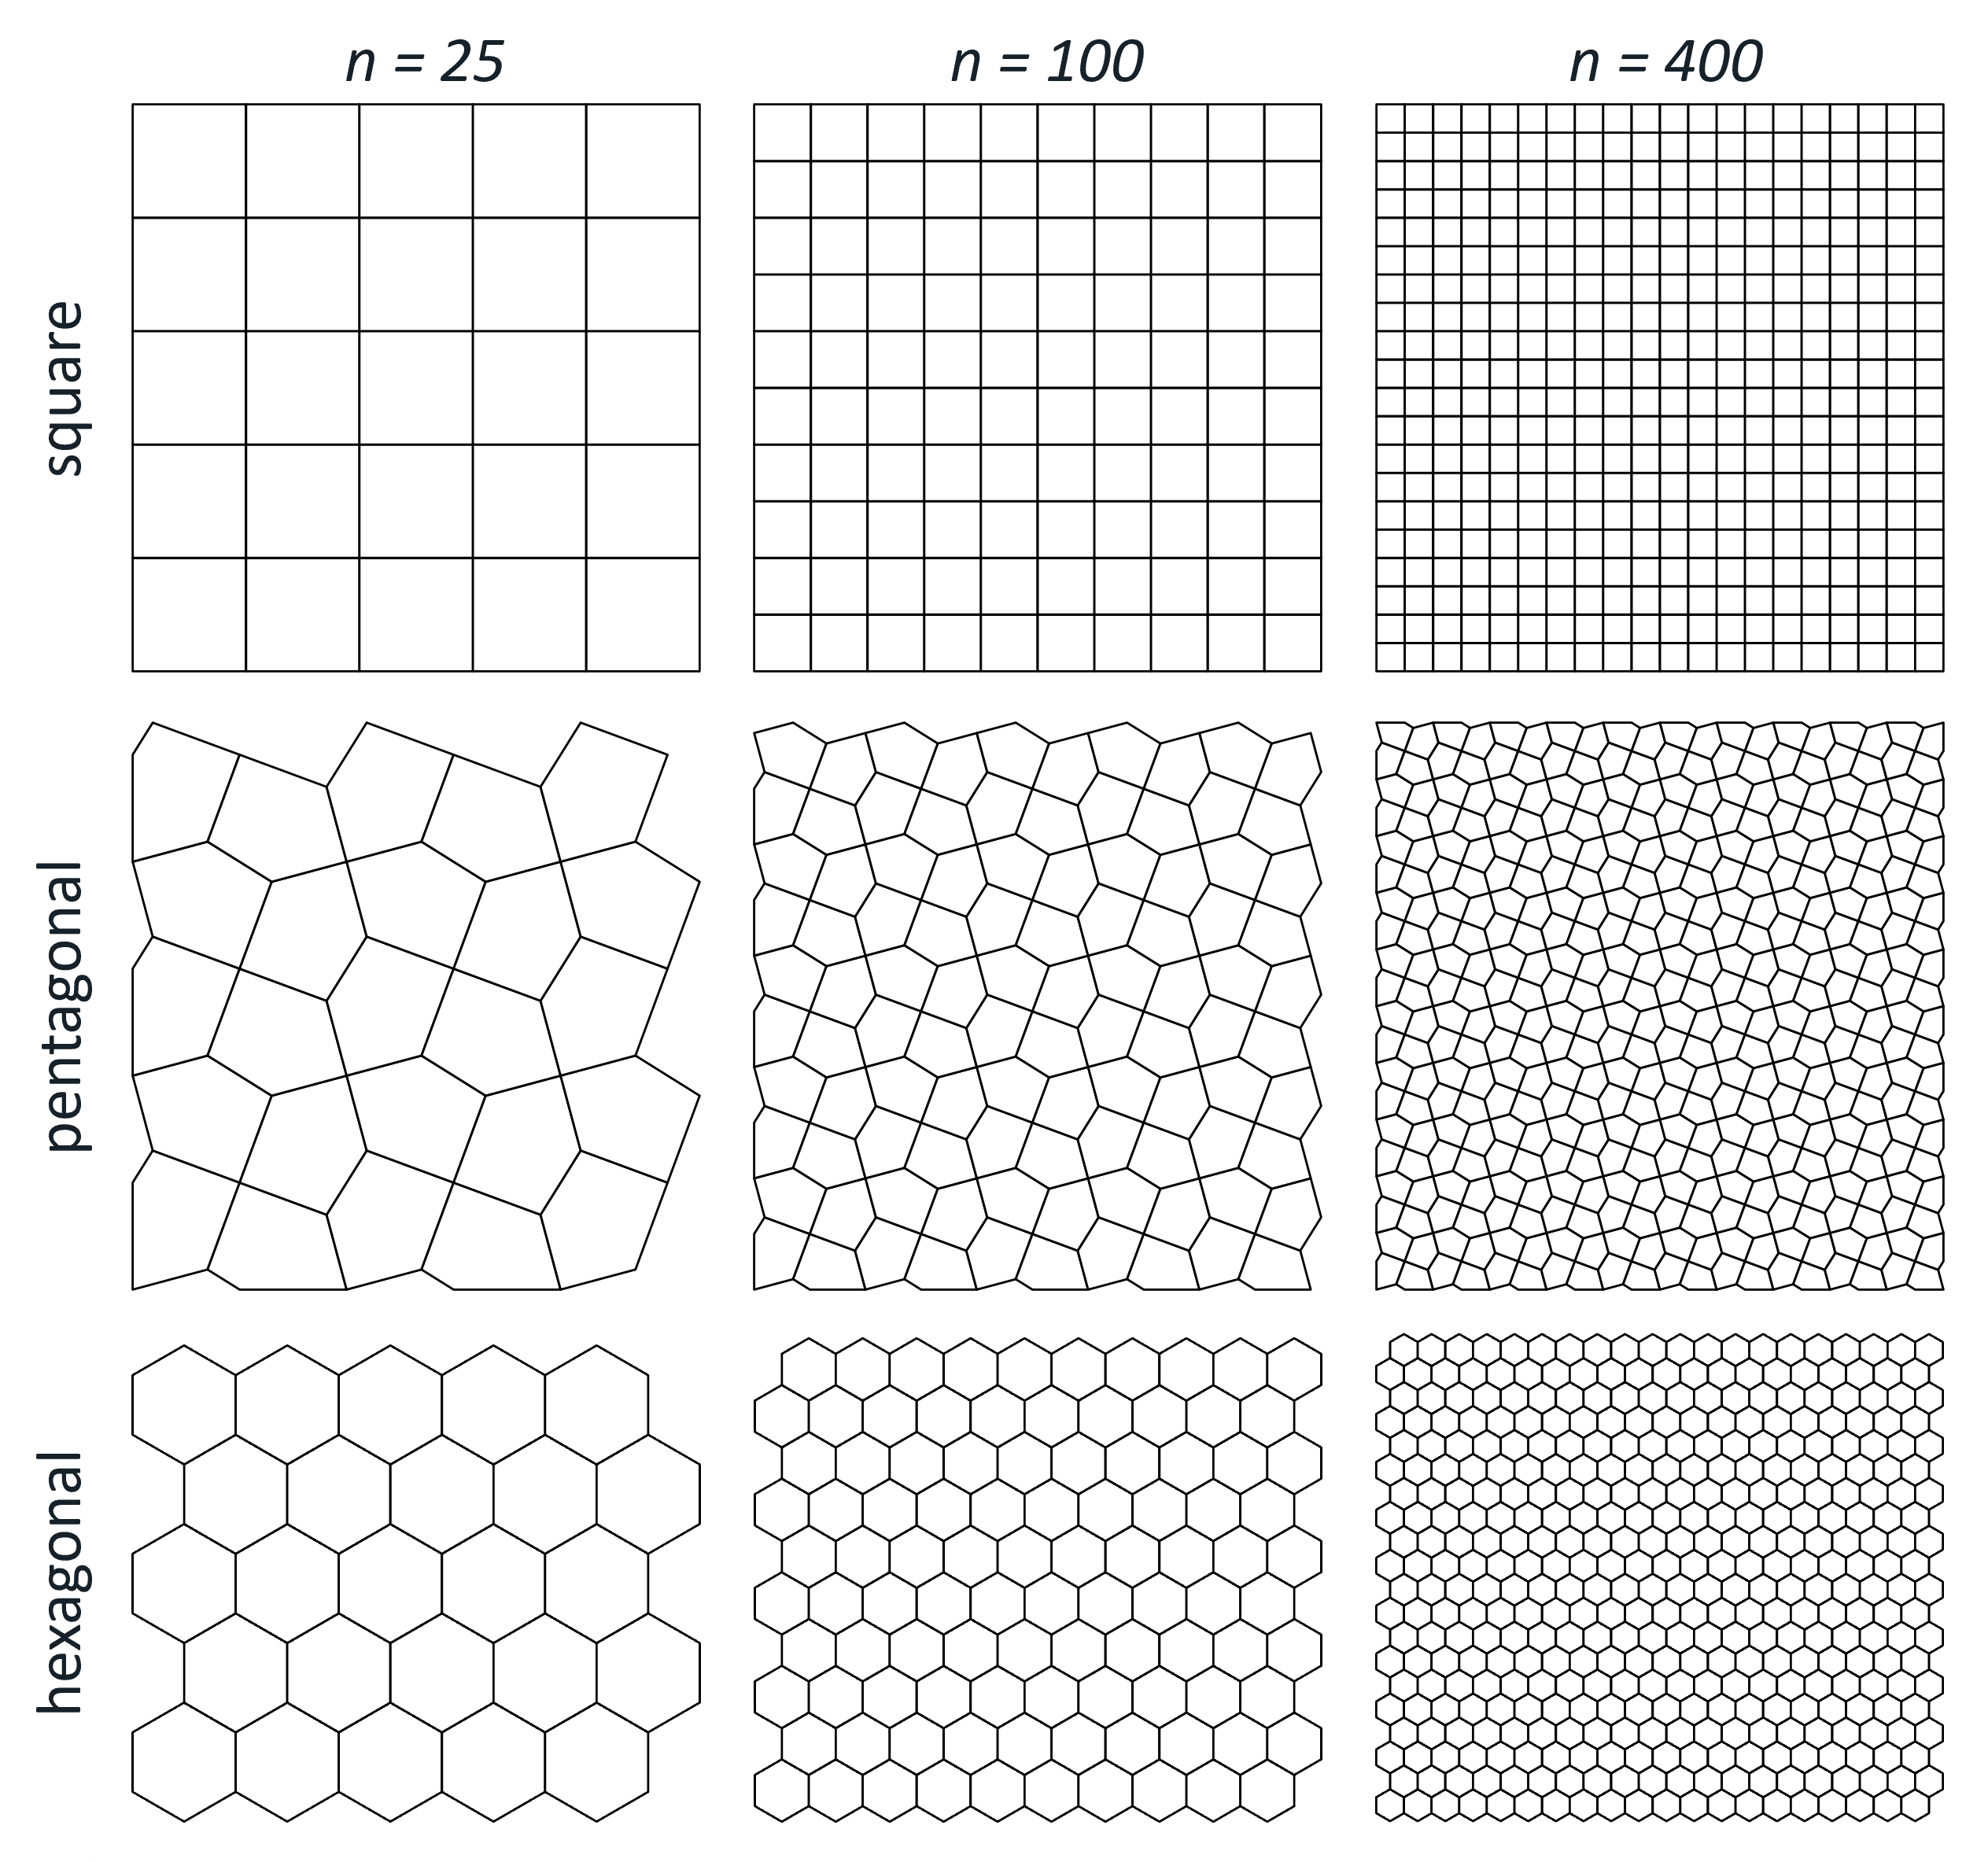
\includegraphics[width=0.6\linewidth,height=\textheight,keepaspectratio]{figures/structures.png}

}

\caption{\label{fig-structures}Simulated data spatial configurations.}

\end{figure}%

\subsection{Synthetic region
delineation}\label{synthetic-region-delineation}

Regions were predefined on all three geometries at two dataset sizes:
\(n=100\) and \(n=400\), giving six spatial configurations in total. For
each spatial configuration, five polygons were randomly selected as
seeds, which grow into spatially connected regions, folowing the
procedure of \citet{guo2023}. The process was repeated 10 times per
configuration, producing 10 distinct zonations. The minimum region size
was set to 12 polygons for \(n = 100\) and 48 polygons for \(n = 400\).
These zonations are utilized in contiguity corruption parametrization
and they provide the basis for generating synthetic attribute data for
the regionalization experiment.

\subsection{Contiguity corruption}\label{contiguity-corruption}

To simulate the effect of topological errors on spatial analysis, a
controlled procedure for corrupting the Rook contiguity spatial weights
matrix \(W\) was developed. Starting from a topologically valid graph,
edges (i.e., adjacency relationships between polygons) are iteratively
removed to progressively degrade the spatial neighbourhood structure.
Missing adjacencies are distributed spatially according to three
distinct patterns:

\begin{itemize}
\tightlist
\item
  \textbf{Randomly:} Edges are removed uniformly at random across the
  entire graph, representing spatially unpatterned errors with no
  particular spatial structure.
\item
  \textbf{Region borders:} Only edges crossing the boundary between two
  predefined regions can be removed, simulating errors arising from the
  integration of independently digitised datasets.
\item
  \textbf{Local:} Edges within or immediately adjacent to a single
  predefined region are targeted, representing localised digitisation or
  editing errors.
\end{itemize}

\begin{figure}

\centering{

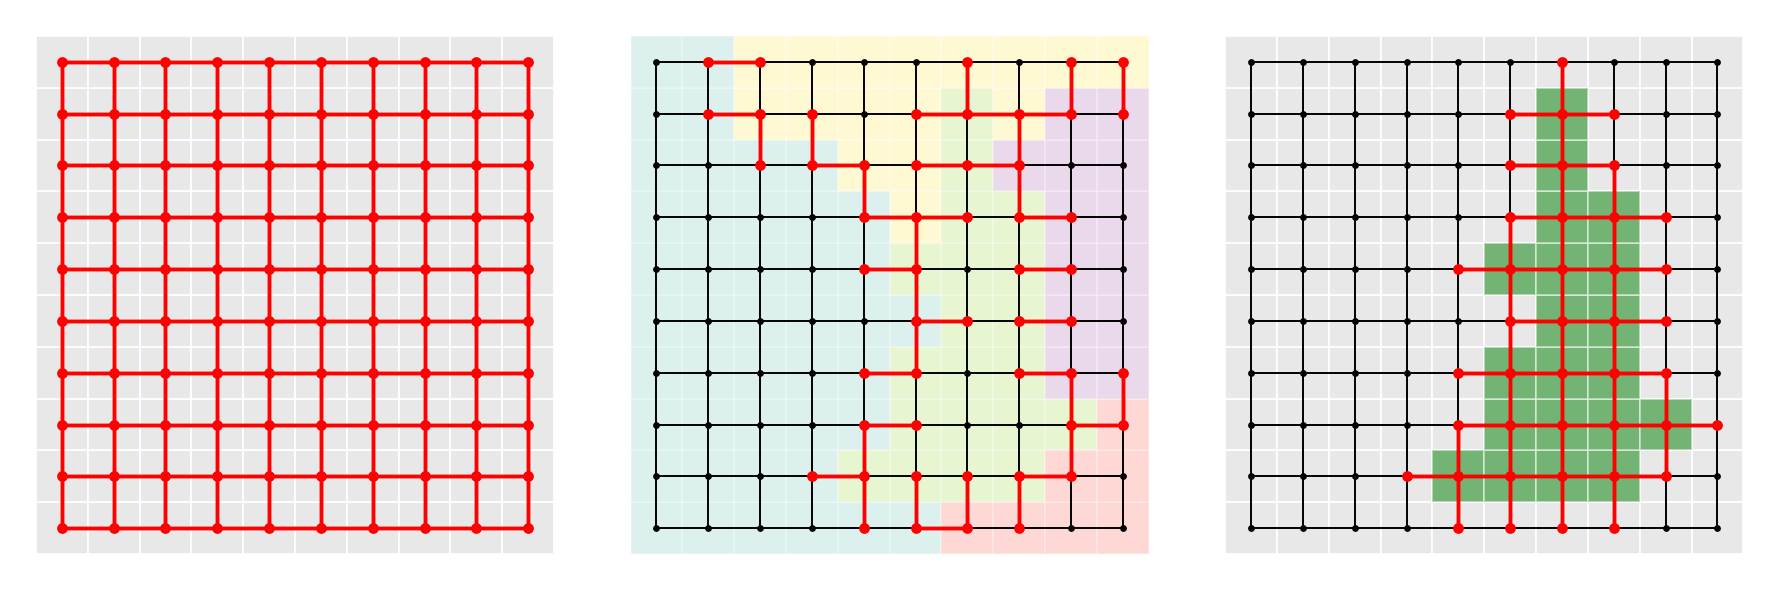
\includegraphics[width=0.8\linewidth,height=\textheight,keepaspectratio]{figures/cor_method.png}

}

\caption{\label{fig-cor_method}Deletable edges (highlighted in red):
random (left), region borders (center), local (right)}

\end{figure}%

Since spatial autocorrelation measures aren't explicitely defined for
observations with no neighbours (isolates), their occurence has to be
prevented while corrupting \(W\). If at least one of two observations
connected by an edge has a node degree of 1 (has only 1 neigbour), the
edge is not eligible for removal. Similarly, regionalization algorithms
require a single connected component, edges whose removal would
disconnect the graph, referred to as bridges, cannot be removed.

-maximally corrupted graph no isolates/mst

At each iteration, the set of removable edges is computed as the
intersection of the method-eligible and constraint-eligible subgraphs.
One edge is removed, the constraint set is recomputed, and the process
repeats until no further deletions are possible. From this sequence, 19
graphs were selected to represent a linear progression of missing edges,
culminating in the maximally corrupted graph. Each sequence is repeated
10 times, yielding 190 corrupted graphs per corruption method. For the
region borders and local corruption methods, each of the 10 repetitions
is paired with a distinct zonation.

To avoid circularity in the regionalization evaluation, any corrupted
graph derived from a given zonation is excluded from experiments if the
input data were generated based on the same zonation.

\subsection{Spatial autocorrelation
workflow}\label{spatial-autocorrelation-workflow}

\subsubsection{Synthetic data}\label{synthetic-data}

Attribute values were generated through a pure spatial autoregressive
(SAR) process, following the procedure in
\citet{floraxImpactsMisspecifiedSpatial1995}:

\[y=(I-\rho W)^{-1} \epsilon\]

where \(y\) is the resulting vector of generated attribute values, \(I\)
is a identity matrix, \(\rho\) is the spatial autoregressive parameter,
\(W\) is row-standartized Rook contiguity spatial weight matrix derived
from each spatial configuration and \(\epsilon\) is random normal error
vector. The parameter \(\rho\) was varied from -0.9 to 0.9 in increments
of 0.1, with 10 independent draws of \(\epsilon\) per value of \(\rho\).
This produced 190 unique value datasets per spatial configuration
representing a wide spectrum differently spatially autocorrelated
datasets (see examples in Figure~\ref{fig-sar_examples}).

\begin{figure}

\centering{

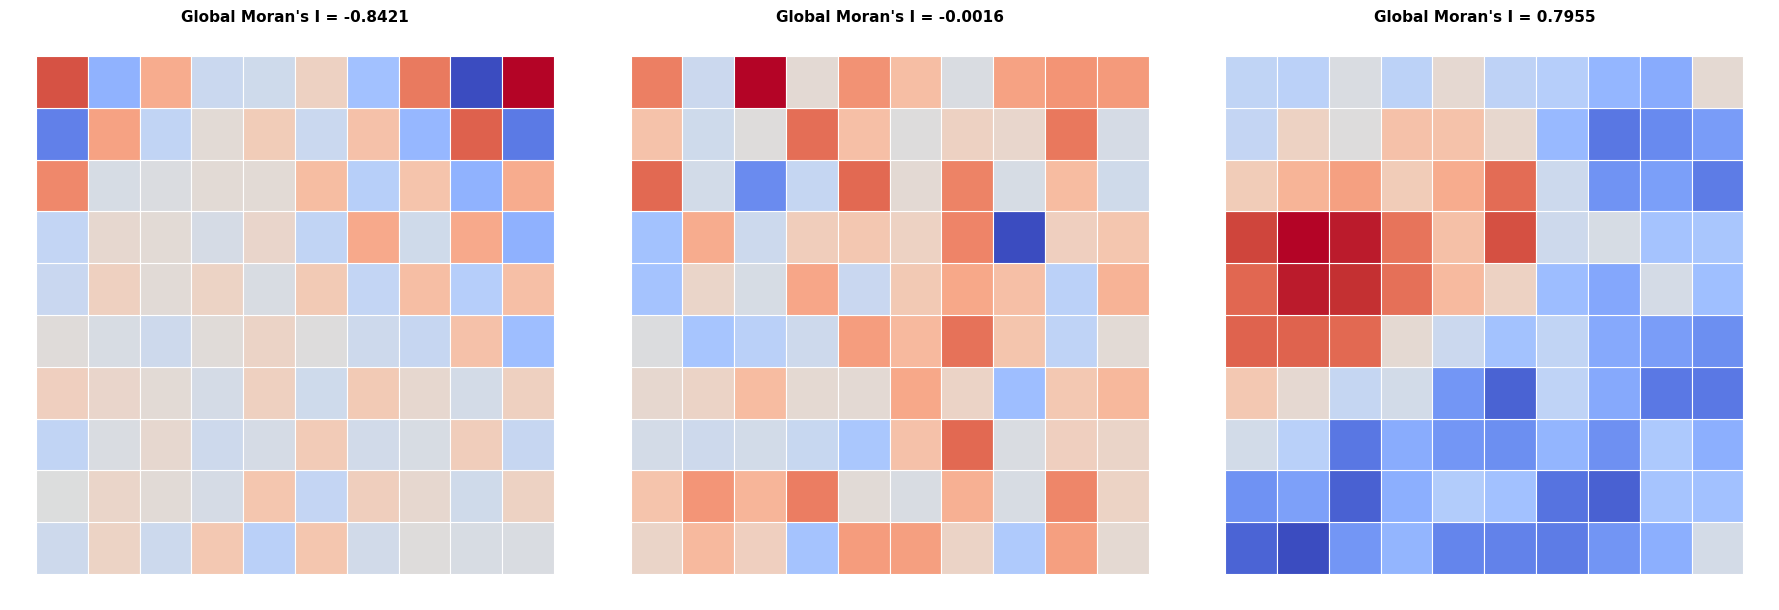
\includegraphics[width=0.8\linewidth,height=\textheight,keepaspectratio]{figures/moran_extremes.png}

}

\caption{\label{fig-sar_examples}Examples of generated SAR data.}

\end{figure}%

\subsubsection{Real data}\label{real-data}

-us election counties (3k)

-guerry (85)

-sacramento1 (403)

\subsubsection{Computation}\label{computation}

\subsubsection{Evaluation}\label{evaluation}

\subsection{Regionalization workflow}\label{regionalization-workflow}

\subsubsection{Synthetic data}\label{synthetic-data-1}

Tgenerated to exhibit strict stratified heterogeneity, meaning that true
regression coefficients are constant within each predefined region but
differ across regions. The underlying data-generating process follows a
simple linear regression model used in \citet{guo2023}:

\[y = \beta_0 + \beta_1 x_1 + \beta_2 x_2 + \epsilon\]

where \(x_1, x_2 \sim \mathcal{U}[0, 1)\) are independent covariates
drawn i.i.d. from a uniform distribution,
\(\epsilon \sim \mathcal{N}(0, \sigma^2)\) is a random error term with
\(\sigma = 0.1\), and \(\beta_0\), \(\beta_1\), \(\beta_2\) are
region-specific regression coefficients. Within each of the five
predefined regions, \(\beta_1\) and \(\beta_2\) take distinct values
drawn from \(\{-2, -1, 0, 1, 2\}\), while \(\beta_0 = 0\) in all
regions.

For each zonation, five independent sets of attribute values were
generated following this process and subsequently used as input to the
regionalization algorithms.

\subsubsection{Real data}\label{real-data-1}

-ceara zika (184)

-chicago airbnb (77)

-south (1k+)

\subsubsection{Computation}\label{computation-1}

\subsubsection{Evaluation}\label{evaluation-1}

-ARI

-FN/FP counts?

\section{Results}\label{results}

\subsection{Spatial autocorrelation}\label{spatial-autocorrelation-1}

\subsubsection{Global}\label{global}

-poster

\subsubsection{Local}\label{local}

-ubytek lisa clusteru?

\subsection{Regionalization}\label{regionalization-1}

-skater je vic sensitive u synthetic dat, ale u real je to dost random

-borders seem to delat vetsi mess

\renewcommand\refname{Discussion}
\bibliography{reference.bib}

\end{document}
